\textbf{Solution:}

\noindent
Let's perform an initial simplification:

\begin{multicols}{2}
\textbf{For D0:}
\begin{align*}
    D0 &= !Q0 \cdot !Q1 \cdot !Q2 \cdot !IL1 \cdot IL0 + \\
       &\quad !Q0 \cdot Q1 \cdot Q2 \cdot IL1 \cdot !IL0 + \\
       &\quad Q0 \cdot !Q1 \cdot !Q2 \cdot !IL1 \cdot IL0 + \\
       &\quad Q0 \cdot Q1 \cdot Q2 \cdot IL1 \cdot !IL0 \\
    &= !Q1 \cdot !Q2 \cdot !IL1 \cdot IL0 + \\
    &\quad Q1 \cdot Q2 \cdot IL1 \cdot !IL0 \\
    \text{where} \\
    IL1 &= input\_leftright1 \\
    IL0 &= input\_leftright0 \\
    IS &= input\_speed
\end{align*}
\columnbreak
\begin{figure}[H]
    \centering
    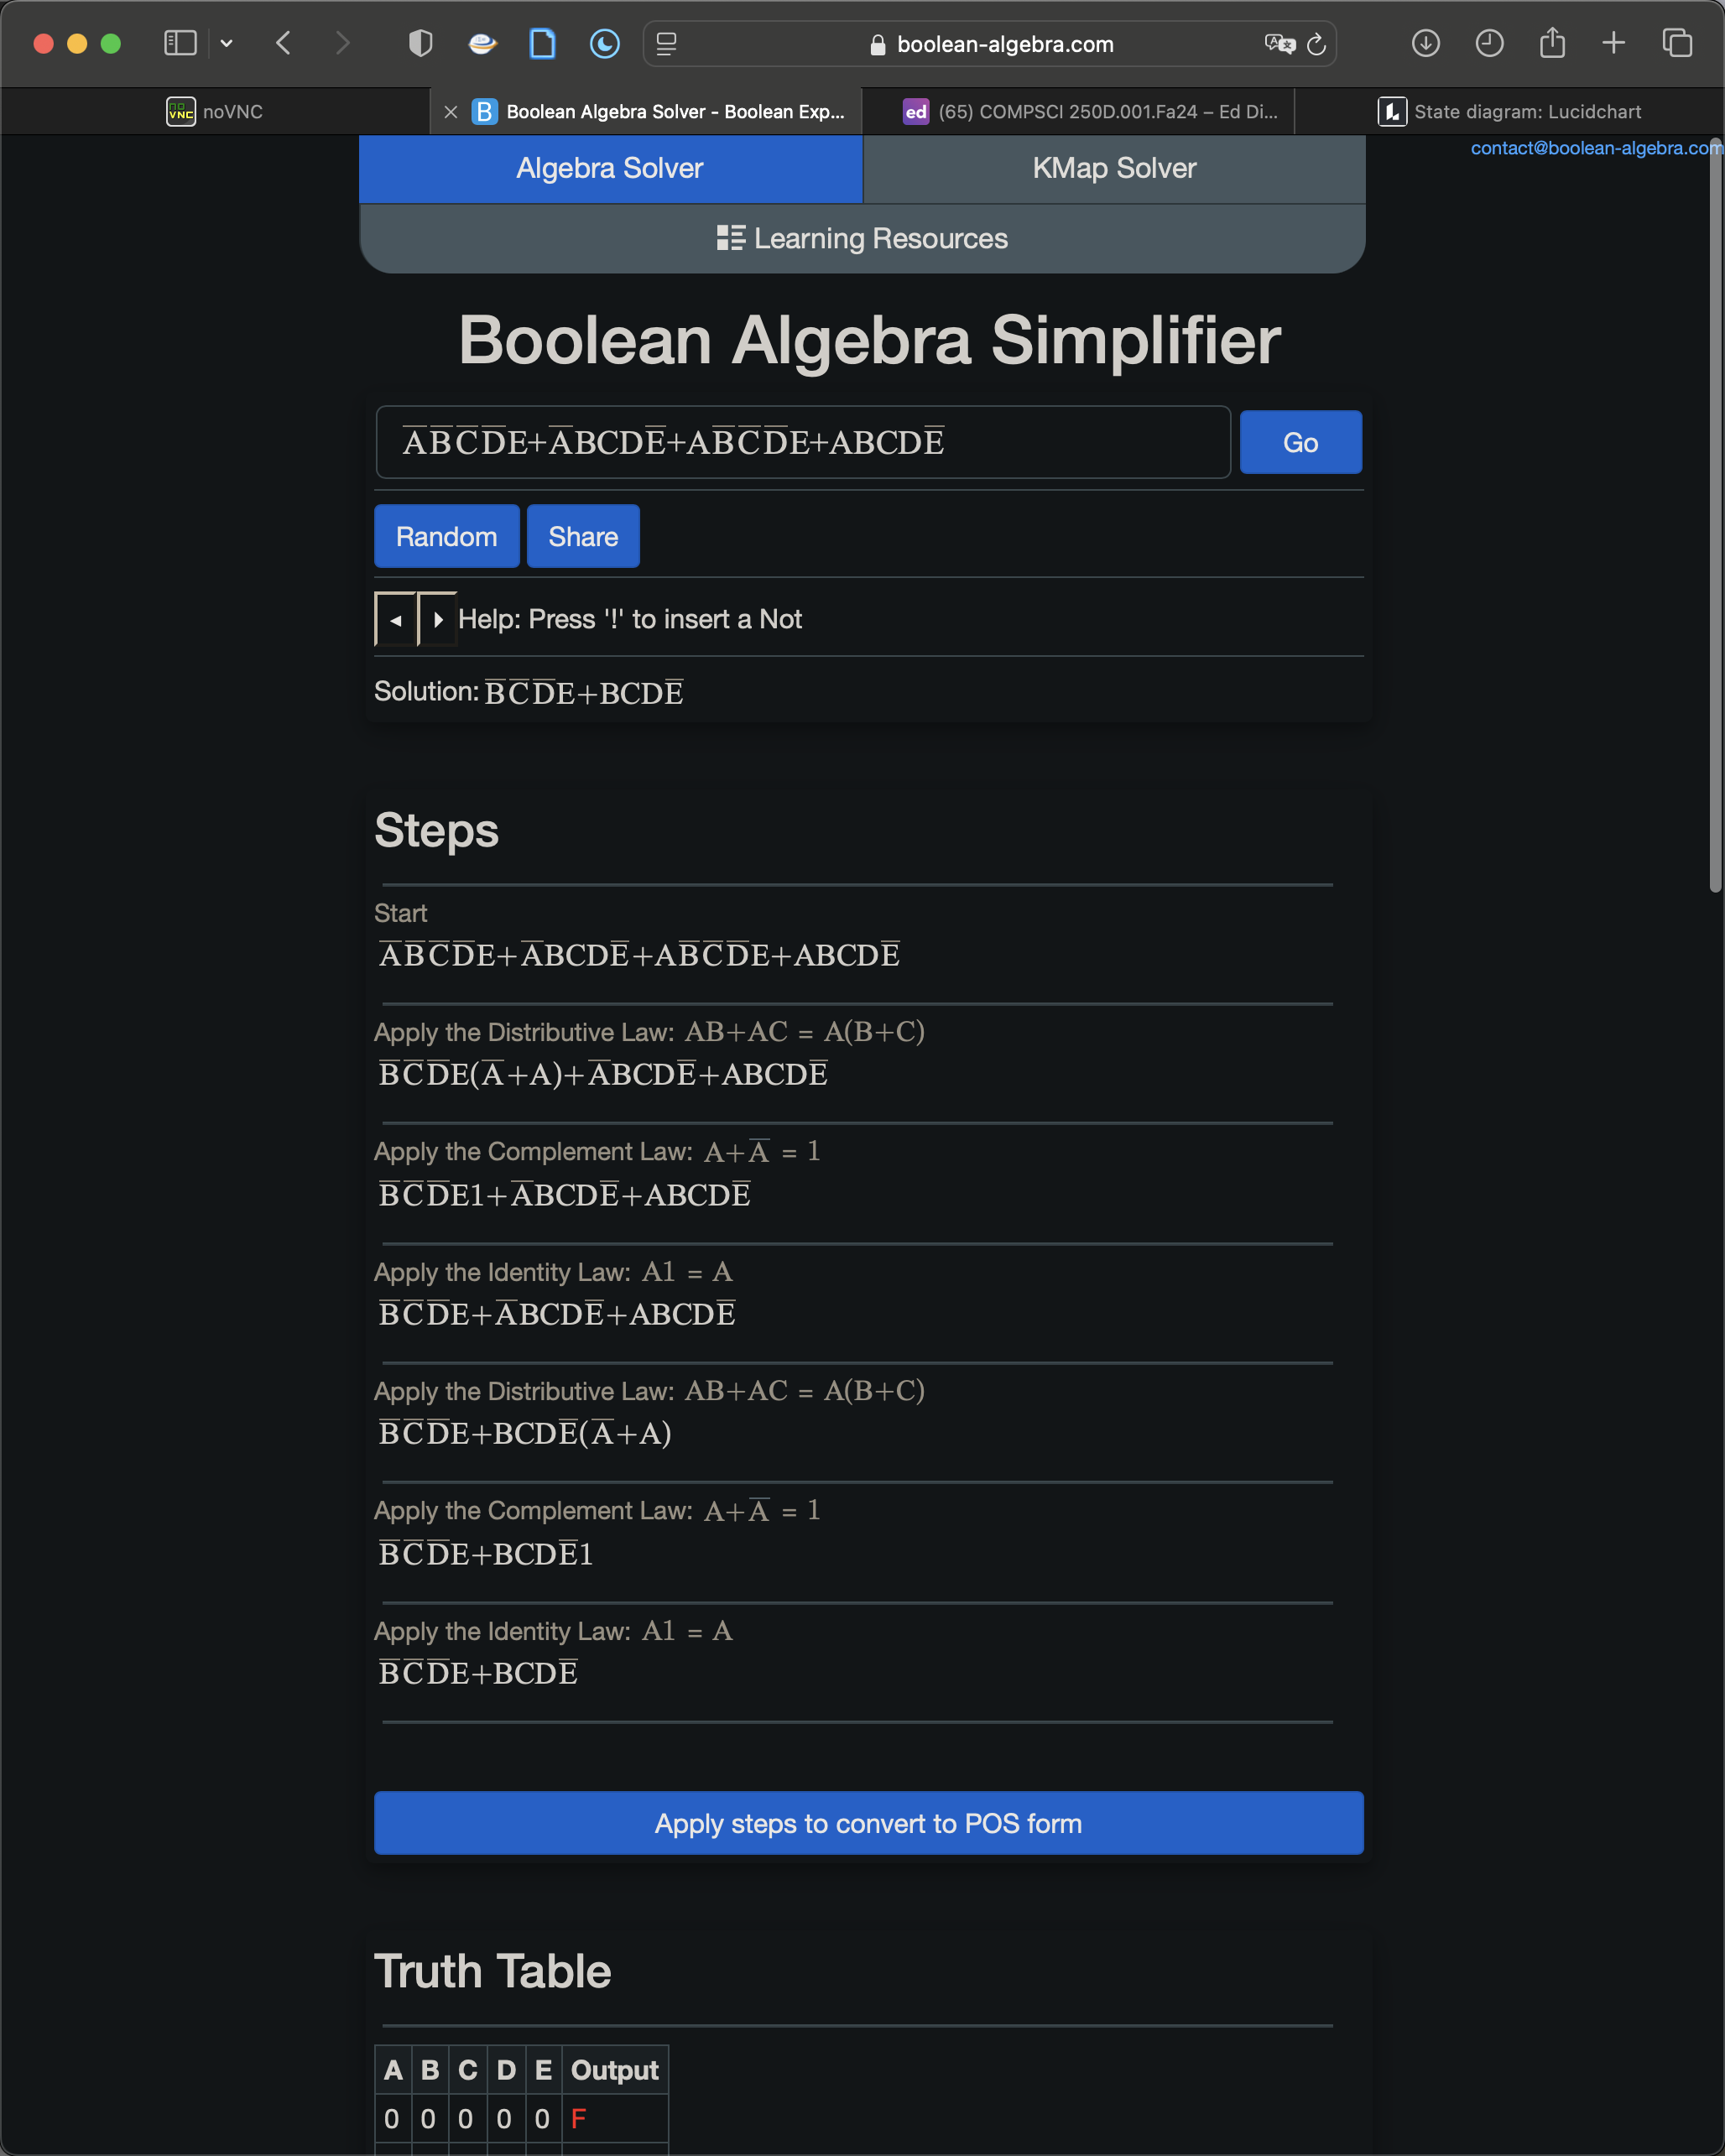
\includegraphics[width=0.66\linewidth]{figures/D0simp.png}
    \caption{Simplified Boolean expression for D0 (simplified using Boolean algebra \cite{boolean-algebra})}
\end{figure}
\end{multicols}

\begin{multicols}{2}
    \textbf{For D1:}
    \begin{align*}
        D1 &=     !Q0 \cdot !Q1 \cdot !Q2 \cdot  IL1 \cdot !IL0 \cdot  IS + \\
           &\quad !Q0 \cdot !Q1 \cdot  Q2 \cdot  IL1 \cdot !IL0 \cdot !IS + \\
           &\quad !Q0 \cdot !Q1 \cdot  Q2 \cdot  IL1 \cdot !IL0 \cdot  IS + \\
           &\quad !Q0 \cdot  Q1 \cdot !Q2 \cdot !IL1 \cdot !IL0 + \\
           &\quad !Q0 \cdot  Q1 \cdot !Q2 \cdot  IL1 \cdot !IL0 + \\
           &\quad !Q0 \cdot  Q1 \cdot  Q2 \cdot !IL1 \cdot !IL0 + \\
           &\quad !Q0 \cdot  Q1 \cdot  Q2 \cdot !IL1 \cdot  IL0 \cdot !IS + \\
           &\quad !Q0 \cdot  Q1 \cdot  Q2 \cdot  IL1 \cdot !IL0 + \\
           &\quad  Q0 \cdot !Q1 \cdot !Q2 \cdot  IL1 \cdot !IL0 \cdot  IS + \\
           &\quad  Q0 \cdot  Q1 \cdot  Q2 \cdot !IL1 \cdot !IL0 + \\
           &\quad  Q0 \cdot  Q1 \cdot  Q2 \cdot !IL1 \cdot  IL0 \cdot !IS + \\
           &\quad  Q0 \cdot  Q1 \cdot  Q2 \cdot  IL1 \cdot !IL0 \\
           &\text{(SEE NEXT PAGE)}
    \end{align*}
\end{multicols}

\newpage

\begin{multicols}{2}
    \begin{align*}
        &=     !Q1 \cdot !Q2 \cdot  IL1 \cdot !IL0 \cdot  IS + \\
        &\quad !Q0 \cdot !Q1 \cdot  Q2 \cdot  IL1 \cdot !IL0 + \\
        &\quad !Q0 \cdot  Q1 \cdot !Q2 \cdot !IL0 + \\
        &\quad  Q1 \cdot  Q2 \cdot (!IL0 + !IL1 \cdot !IS)  \text{(by myself)}\\
    &=     !Q1 \cdot !Q2 \cdot  IL1 \cdot !IL0 \cdot  IS + \\
    &\quad !Q0 \cdot !Q1 \cdot  Q2 \cdot  IL1 \cdot !IL0 + \\
    &\quad !Q0 \cdot  Q1 \cdot !IL0 + \\
    &\quad  Q1 \cdot  Q2 \cdot (!IL0 + !IL1 \cdot !IS) \\
        &=     !Q1 \cdot !Q2 \cdot  IL1 \cdot !IL0 \cdot  IS + \\
        &\quad !Q0 \cdot  Q2 \cdot  IL1 \cdot !IL0 + \\
        &\quad !Q0 \cdot  Q1 \cdot !IL0 + \\
        &\quad  Q1 \cdot  Q2 \cdot (!IL0 + !IL1 \cdot !IS) \text{(by myself)}\\
    \end{align*}
    \columnbreak
    \begin{figure}[H]
        \centering
        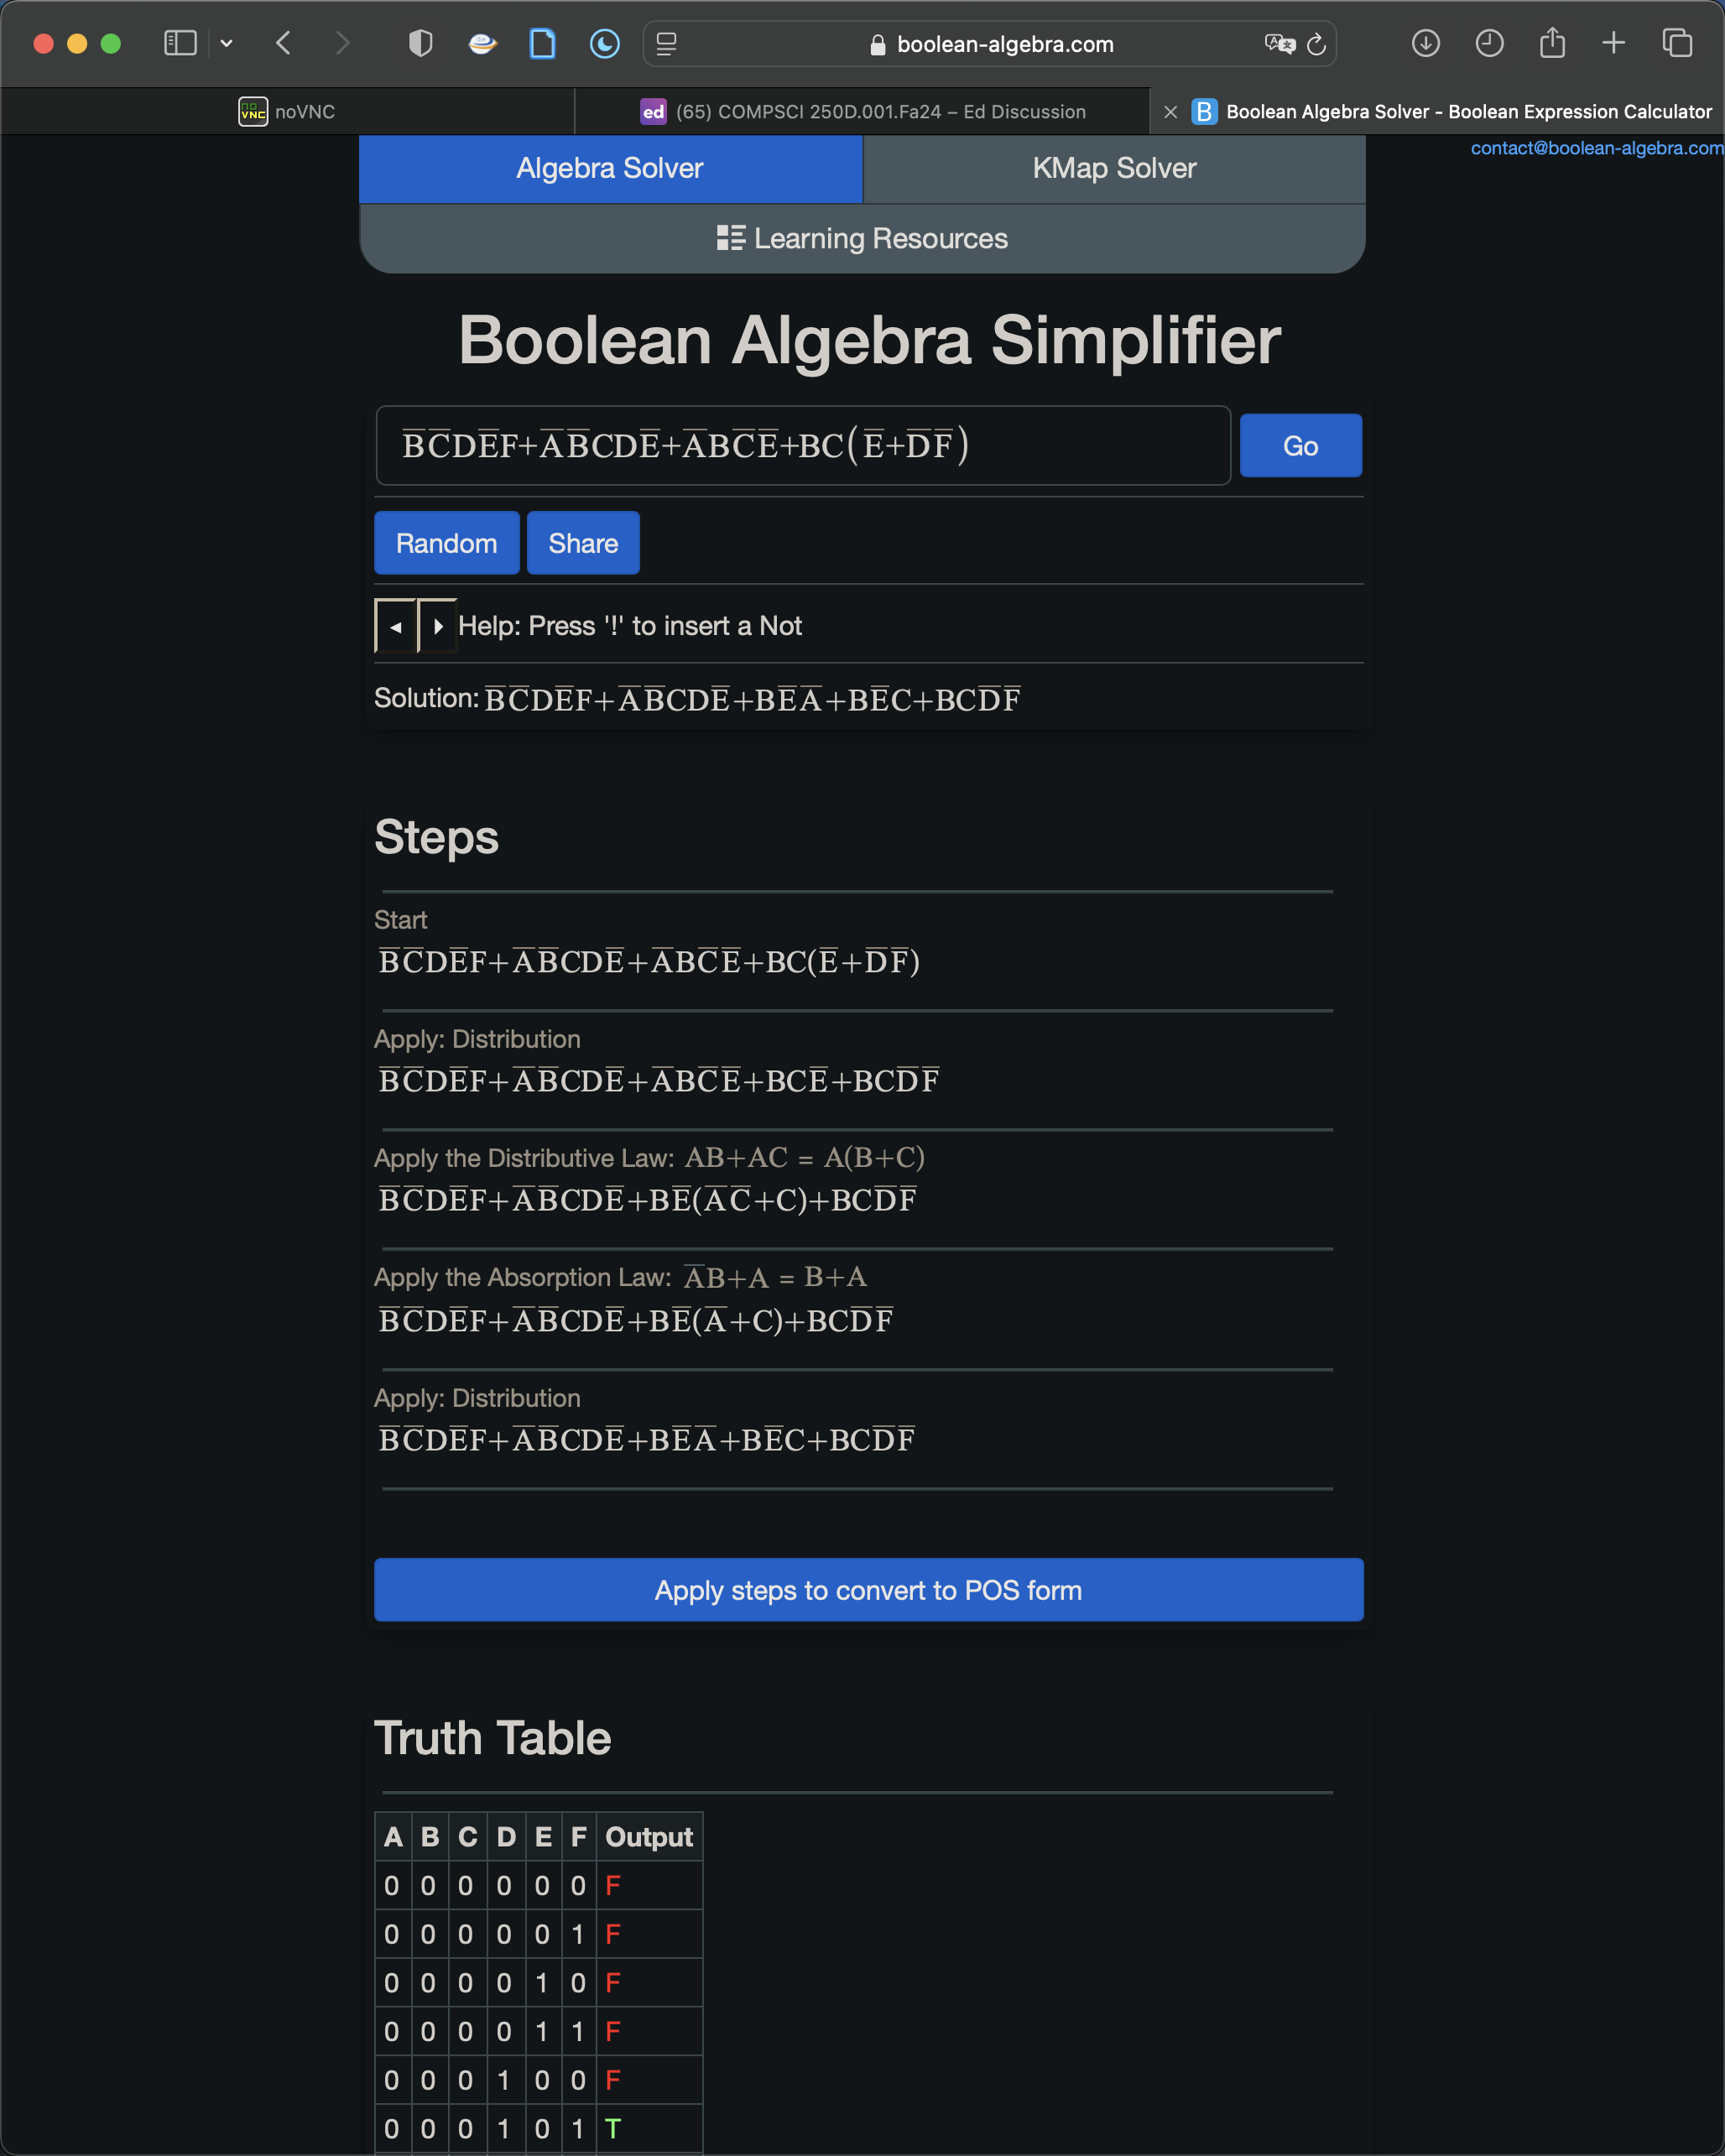
\includegraphics[width=0.66\linewidth]{figures/D1simp.png}
        \caption{Simplified Boolean expression for D1 (simplified using Boolean algebra \cite{boolean-algebra})}
    \end{figure}
\end{multicols}

\begin{multicols}{2}
    \textbf{For D2:}
    \begin{align*}
        D2  &=     !Q0 \cdot !Q1 \cdot !Q2 \cdot  IL1 \cdot !IL0 \cdot !IS + \\
            &\quad !Q0 \cdot !Q1 \cdot  Q2 \cdot !IL1 \cdot !IL0 + \\
            &\quad !Q0 \cdot !Q1 \cdot  Q2 \cdot  IL1 \cdot !IL0 \cdot  IS + \\
            &\quad !Q0 \cdot  Q1 \cdot !Q2 \cdot !IL1 \cdot  IL0 \cdot !IS + \\
            &\quad !Q0 \cdot  Q1 \cdot !Q2 \cdot  IL1 \cdot !IL0 + \\
            &\quad !Q0 \cdot  Q1 \cdot  Q2 \cdot !IL1 \cdot !IL0 + \\
            &\quad !Q0 \cdot  Q1 \cdot  Q2 \cdot !IL1 \cdot  IL0 \cdot  IS + \\
            &\quad !Q0 \cdot  Q1 \cdot  Q2 \cdot  IL1 \cdot !IL0 + \\
            &\quad  Q0 \cdot !Q1 \cdot !Q2 \cdot  IL1 \cdot !IL0 \cdot !IS + \\
            &\quad  Q0 \cdot  Q1 \cdot  Q2 \cdot !IL1 \cdot !IL0 + \\
            &\quad  Q0 \cdot  Q1 \cdot  Q2 \cdot !IL1 \cdot  IL0 \cdot  IS + \\
            &\quad  Q0 \cdot  Q1 \cdot  Q2 \cdot  IL1 \cdot !IL0 \\
           &=     !Q1 \cdot !Q2 \cdot  IL1 \cdot !IL0 \cdot !IS + \\
           &\quad !Q0 \cdot  Q2 \cdot (!IL1 \cdot !IL0 + !IL0 \cdot  IS) + \\
           &\quad !Q0 \cdot  Q1 \cdot !Q2  \cdot !IL1 \cdot  IL0 \cdot !IS + \\
           &\quad !Q0 \cdot  Q1 \cdot  IL1 \cdot !IL0 + \\
           &\quad  Q1 \cdot  Q2 \cdot (!IL0 + !IL1 \cdot  IS) \text{(by myself)} \\
        % &=     !Q1 \cdot !Q2 \cdot  IL1 \cdot !IL0 \cdot  IS + \\
        % &\quad !Q0 \cdot !Q1 \cdot  Q2 \cdot  IL1 \cdot !IL0 + \\
        % &\quad !Q0 \cdot  Q1 \cdot !IL0 + \\
        % &\quad  Q1 \cdot  Q2 \cdot (!IL0 + !IL1 \cdot !IS) \\
        %     &=     !Q1 \cdot !Q2 \cdot  IL1 \cdot !IL0 \cdot  IS + \\
        %     &\quad !Q0 \cdot  Q2 \cdot  IL1 \cdot !IL0 + \\
        %     &\quad !Q0 \cdot  Q1 \cdot !IL0 + \\
        %     &\quad  Q1 \cdot  Q2 \cdot (!IL0 + !IL1 \cdot !IS) \text{(by myself)}\\
        \end{align*}
        \columnbreak
        % \begin{figure}[H]
        %     \centering
        %     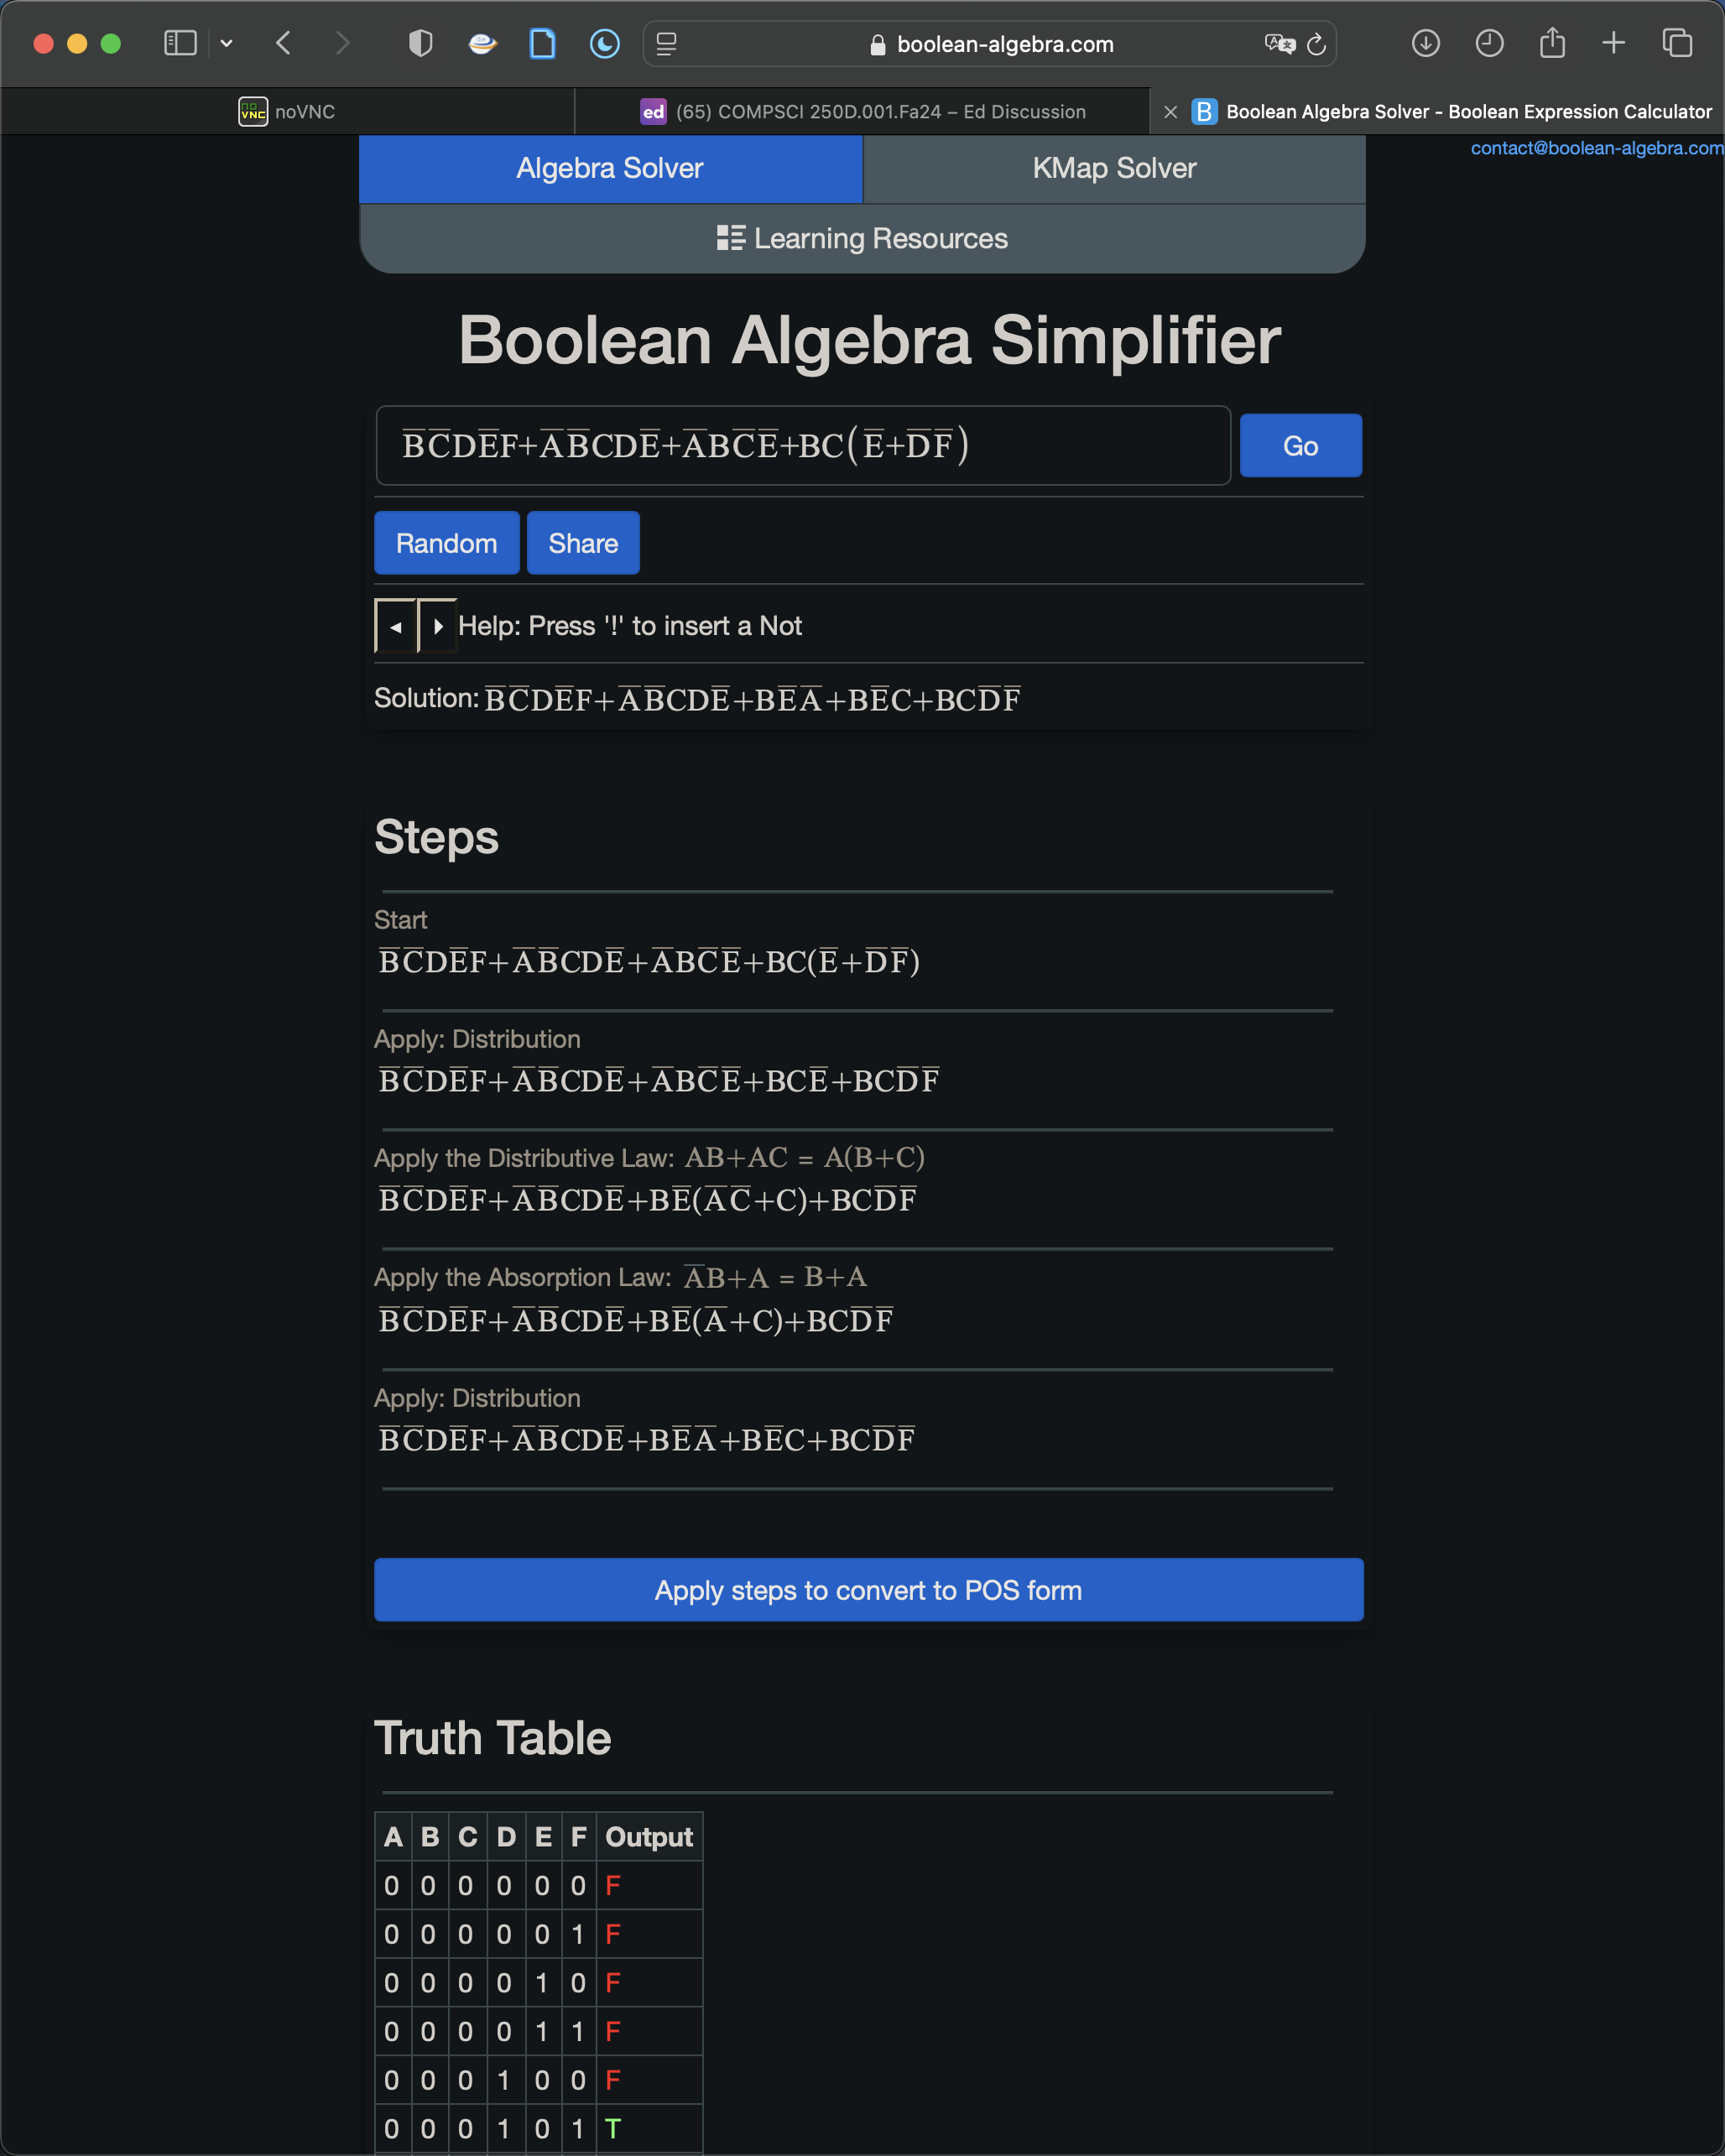
\includegraphics[width=0.66\linewidth]{figures/D1simp.png}
        %     \caption{Simplified Boolean expression for D1 (simplified using Boolean algebra \cite{boolean-algebra})}
        % \end{figure}
    \end{multicols}

\newpage

\noindent
The logic expression of output bits are obivious:

\begin{align*}
    \text{out\_blocked} &=  Q0 \\
    \text{out\_posision1} &= Q1 \\
    \text{out\_posision0} &= Q2
\end{align*}


\newpage
% ----------------------------------------------------------------
% Drafted by Juntang Wang 2024-10-22
% ----------------------------------------------------------------  
